\documentclass[12pt,twoside]{article}
\usepackage{jmlda}
\usepackage[square,sort,comma,numbers]{natbib}
\usepackage{bm}
\newcommand{\cyrchar}[1]{\foreignlanguage{russian}{#1}}
\usepackage{caption}
%\NOREVIEWERNOTES
\title
    [Предсказание показания фМРТ по видео, показанному человеку] % Краткое название; не нужно, если полное название влезает в~колонтитул
    {Предсказание показания фМРТ по видео, показанному человеку}
\author
    [Дорин~Д.\,Д.] % список авторов для колонтитула; не нужен, если основной список влезает в колонтитул
    {Дорин~Д.\,Д., Киселев~Н.\,С., Грабовой~А.\,В.} % основной список авторов, выводимый в оглавление
    [Дорин~Д.\,Д.$^{1,2}$, Грабовой~А.\,В.$^2$] % список авторов, выводимый в заголовок; не нужен, если он не отличается от основного

\email
    {dorin.dd@phystech.edu}
\organization
    {$^1$Организация; $^2$Организация}
\abstract
    {Исследуется задача прогнозирования показаний датчиков фМРТ по видеоряду, 
    показанному человеку. 
    Предложен метод апроксимации показаний фМРТ по видеоряду на основе моделей типа Трансформер. 
    Проанализирована зависимость между показаниями датчиков и восприятием внешнего мира человеком.
    Эффективность предложенного подхода демонстрируется на наборе данных, 
    собранных у большой группы людей в процессе просмотра фильма.

\bigskip
\textbf{Ключевые слова}: \emph {фМРТ, видеоряд, Трансформер модель}.}
\titleEng
    {JMLDA paper example: file jmlda-example.tex}
\authorEng
    {Author~F.\,S.$^1$, CoAuthor~F.\,S.$^2$, Name~F.\,S.$^2$}
\organizationEng
    {$^1$Organization; $^2$Organization}
\abstractEng
    {This document is an example of paper prepared with \LaTeXe\
    typesetting system and style file \texttt{jmlda.sty}.
    
\bigskip
\textbf{Keywords}: \emph{keyword, keyword, more keywords}.}

\begin{document}
\maketitle
%\linenumbers
\section{Введение}
Человеческий мозг~--- один из самых интересных объектов исследования \citep{Zhumakova}. 
Внутречерепные записи человека являются редким и ценным источником информации о мозге.
Поэтому изучение методов прогнозирования данных о функциональной активности коры головного мозга является актуальной темой в настоящее время.

Функциональная магнитно-резонансная томография, далее~--- фМРТ \citep{Ushakov},~--- один из методов исследования активности головного мозга.
фМРТ проводится с целью измерения гемодинамических реакций~--- изменений в потоке крови. 
Этот метод основывается на связи мозгового кровотока и активности нейронов. Когда область мозга активна, 
приток крови к этой области также увеличивается. 
фМРТ позволяет определить активацию определенной области головного мозга во время нормального функционирования под 
влиянием различных заданий, например, зрительных, когнитивных,  моторных,  речевых.
В работе \citep{Belyaevskaya2018} собраны современные возможности фМРТ в нейровизуализации. 
Под нейровизуализацией понимается общее название нескольких методов, позволяющих визуализировать структуру, функции и биохимические характеристики мозга.

В работе \citep{Berezutskaya2022} собран обширный набор данных, сотоящий из видеорядов, просмотренных 
человеком, и соответствующих снимков фМРТ. Одна из проблем при работе с данными нейровизуализации~--- шум, вызванный 
дивжением головы, биением сердца, тепловыми эффектами и др. 
В работе \citep{https://doi.org/10.48550/arxiv.1804.10167} рассмотрены подходы к подготовке,
предварительной обработке, шумоподавлению, направленные на устранение артефактов, вредных 
для распознавания образов, а также методы классификации данных нейровизуализации.

Наиболее известные методы обработки видео основаны на 3D свертках. 
Отличие 3D от 2D сверток заключается в одновременной работе с пространственной  
и временной частью информации. Существенный недостаток данных методов~--- 
сильное увеличение числа параметров модели и большие вычислительные затраты.
В работе используется более современная архитектура~--- модель типа Трансформер.
Впервые модель Трансформер была предложена в статье <<Attention Is All You Need>> Ashish Vaswani 
\citep{https://doi.org/10.48550/arxiv.1706.03762}. Архитектура активно применяется в области машинного перевода.
А в 2022 году появилась работа \citep{transformer} на тему адаптации архитектуры Трансформер для работы с видеорядами. 
Данная архитектура учитывает пространственно-временные зависимости и повышает скорость обучения засчет механизма внимания.
Сама модель состоит из кодирующего компонента, декодирующего компонента и связи между ними. Каждый компонент состоит из стека 
энкодеров и декодеров соотвественно \citep{badrinarayanan2017segnet}. 
Входящая последовательность, поступающая в энкодер, сначала проходит через слой внимания, помогающий энкодеру 
посмотреть на другие слова во входящем объеме во время кодирования конкретного элемента. 
Выход слоя внимания отправляется в нейронную сеть прямого распространения. 
Аналогично устроен декодер, за исключением наличия еще одного слоя внимания, помогающего фокусироваться на релевантных элементах.

В данной работе предлагается метод аппроксимации показаний датчиков фМРТ по видеоряду. 
При получении метода использовались два основных предположения. Первая гипотеза заключается в существовании зависимости между результатами фМРТ и просматриваемым фильмом.
Второе предположение заключается в том, что реакция мозга, фиксируемая фМРТ, на информацию, поступающую от органов зрения, происходит не мгновенно, а с некоторой задержкой \citep{Demidov}. 
Полученная в ходе экспериментов корреляционная картина между данными в выборке подтверждает 
зависимость между показаниями фМРТ и восприятием внешнего мира человеком. 

Проверка метода проводится на выборке, представленной в работе \citep{Berezutskaya2022}. 
Набор данных включает в себя в себя записи фМРТ 30 участников в возрасте от 7 до 47 лет во время 
выполнения одинаковой задачи и записи внутричерепной электроэнцефалографии 51 участникa в возрасте от 5 до 55 лет. 


\section{Постановка задачи}
Пусть $\mathbf{\Omega}$~--- видеоряд, $\nu$~--- частота кадров, $t$~--- продолжительность видеоряда:
\begin{equation}
    \bm{\Omega} = (\bm{\omega}_{1}, \dots, \bm{\omega}_{\nu \cdot t}),
\end{equation}
где $\bm{\omega} \in \mathbb{R}^{W_{\bm{\omega}} \times H_{\bm{\omega}} \times C_{\bm{\omega}}}$~--- изображение, $W_{\bm{\omega}}$~---
ширина изображения, $H_{\bm{\omega}}$~--- высота изображения и $C_{\bm{\omega}}$~--- число каналов.

Введем также $\mathcal{S}$~--- последовательность фМРТ снимков,  $\mu$~--- частота снимков:
\begin{equation}
    \mathcal{S} = (\bm{s}_{1}, \dots, \bm{s}_{\mu \cdot t}),
\end{equation}
где $\bm{s} \in \mathbb{R}^{X_{\bm{s}} \times Y_{\bm{s}} \times Z_{\bm{s}}}$~--- фМРТ снимок, $X_{\bm{s}},~Y_{\bm{s}},~Z_{\bm{s}}$~--- размерность одного измерения.

Также считаем, что известно несколько дополнительных измерений фМРТ $\mathcal{S}_0$ того же испытуемого.
Необходимо построить отображение $f$:
\begin{equation}
    f(\bm{\omega}_{1}, \dots, \bm{\omega}_{k_i - \nu \cdot \Delta t}, \mathcal{S}_0) = \bm{s}_i,
\end{equation}
которое учитывает задержку $\Delta t$, между фМРТ картиной и моментом получения информации зрительными органами.
Здесь
\begin{equation}
    \label{k_i}
    k_i = \dfrac{\nu \cdot i}{\mu}
\end{equation}
 номер изображения в момент времени $i$-го снимка фМРТ.
\section{Вычислительный эксперимент}
\subsection{Цель эксперимента}
Построить метод аппроксимации снимка фМРТ по видеоряду и нескольким дополнительным измерениям фМРТ того же испытуемого, который 
учитывает задержку $\Delta t$ между реакцией мозга и моментом получения информации зрительными органами. 
\subsection{Набор данных для базового эксперимента}
Обучение модели проводится на наборе данных четвертого испытуемого, представленном в работе \citep{Berezutskaya2022}. 
Для каждого фиксированного гиперпараметра $\Delta t$ обучающая выборка состоит из $641-\mu \cdot \Delta t$  снимков фМРТ и набора соотвествующих изображений из видеоряда. 
Номера изображений определяются по номеру снимка фМРТ соотвественно формуле \eqref{k_i}.  
\subsection{Базовая модель}
В базовом эксперименте используется линейная модель для прогнозирования снимка фМРТ определенного испытуемого по соответствующему кадру из видеоряда. 
Гиперпараметром модели является задержка $\Delta t$.
Одним из параметров модели является коэффициент сжатия воксельных изображений. 
Для сжатия используется MaxPool3d с целью уменьшения числа подбираемых весов и ускорения процесса обучения соотвественно.
Каждое изображения из обучающей выборки предобработано с помощью ResNet152 и представляет собой вектор $X$ признаков размерности 2048. 
Для восстановления значения в каждом вокселе независимо от других по всему признаковому вектору изображения используется линейная регрессия. 
Целевой переменной является сжатый тензор изображения, представленный вектором $Y$, компоненты которого~--- значения в каждом вокселе.
Результатом работы алгоритма является матрица весов $W$, где каждая строка весов соотвествует определенному вокселю из фМРТ снимка.
Отображение устроено следующим образом:
\begin{equation}
    Y = W \cdot X
\end{equation}
\subsection{Результаты эксперимента}
Ниже приведены результаты работы модели при варьировании гиперпараметра $\Delta t$ с фиксированным коэффициентом сжатия $\mathrm{coef} = 4$. 
\begin{figure}[h!]
    \centering
    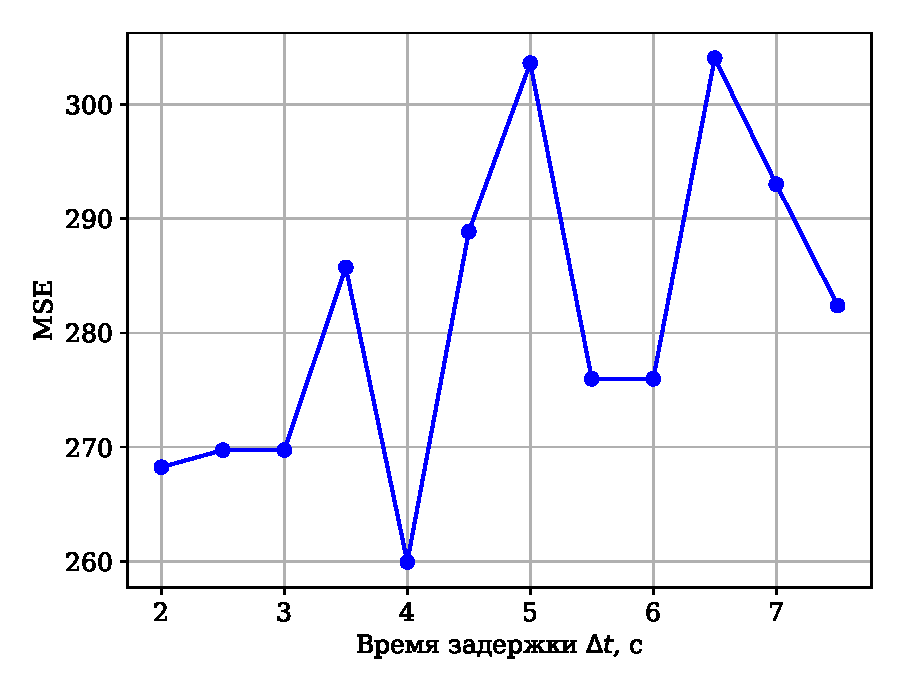
\includegraphics[scale = 0.8]{MSE_dt.eps}
    \caption{Зависимость среднеквадратичной ошибки на тесте от задержки ${\Delta t}$}
    \label{MSE_dt}
\end{figure}

По приведенному графику \ref{MSE_dt} был выбран оптимальный гиперпараметр ${\Delta t}_{opt} = 4$.
В качестве демонстрации работы при оптимальном гиперпараметре ниже приведены срезы оригинального и предсказанного воксельного изображения фМРТ в некоторый момент времени.
\begin{figure}[h]
    \begin{center}
    \begin{minipage}[h]{0.4\linewidth}
    \includegraphics[width=1\linewidth]{sub-04-4-4-5-_-_-orig.eps}
    \caption{Срез оригинального снимка} %% подпись к рисунку
    \label{ris:pred} %% метка рисунка для ссылки на него
    \end{minipage}
    \hfill
    \begin{minipage}[h]{0.4\linewidth}
    \includegraphics[width=1\linewidth]{sub-04-4-4-5-_-_-pred-pg.eps}
    \caption{Срез предсказанного и обработанного снимка}
    \label{ris:pred-pg}
    \end{minipage}
    \end{center}
\end{figure}

\begin{figure}[h!]
    \centering
    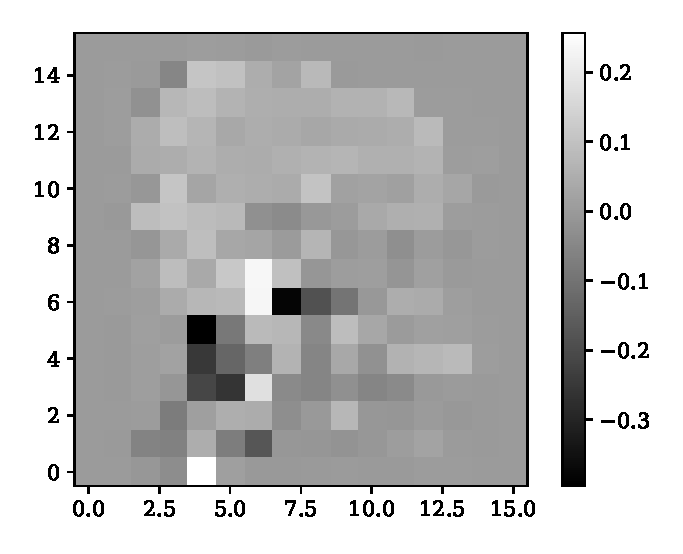
\includegraphics[scale = 0.6]{sub-04-4-4-5-_-_-pred.eps}
    \caption{Срез предсказанного снимка до обработки}
    \label{pred}
\end{figure}

На рисунке \ref{pred} демонстрируется основная проблема модели~--- выбросы, которые портят контрастность изображения.
Перед применением алгоритма была проведена нормализация данных фМРТ.
Поэтому предсказанные значения, не попадающие на отрезок $[0,1]$, считаются антифизичными.
Срез снимка после обработки антифизичных значений в вокселях и применения фильтра Гаусса приведен на рисунке \ref{ris:pred-pg}.
Метрикой оценки качества алгоритма ялвяется среднеквадратичная ошибка.
\begin{table}[H]
    \caption{\label{tab:1} MSE при параметрах модели ${\Delta t}_{opt} = 4$, $\mathrm{coef} = 4$.}
    \begin{center}
    \begin{tabular}{|c|c|}
    \hline
    MSE при обучении & MSE на тесте \\
    \hline
    $253.02$ & $259.92$ \\
    \hline
    \end{tabular}
    \end{center}
\end{table} 
Полученные результаты подтверждают наличие корреляции между снимками фМРТ и изображениями из видеоряда.



\section{Анализ ошибки}

\section{Заключение}



\bibliographystyle{plain}

\bibliography{dorin.bib}

%\begin{thebibliography}{1}

%\bibitem{author09anyscience}
%    \BibAuthor{Author\;N.}
%    \BibTitle{Paper title}~//
%    \BibJournal{10-th Int'l. Conf. on Anyscience}, 2009.  Vol.\,11, No.\,1.  Pp.\,111--122.
%\bibitem{myHandbook}
%    \BibAuthor{Автор\;И.\,О.}
%    Название книги.
%    Город: Издательство, 2009. 314~с.
%\bibitem{author09first-word-of-the-title}
%    \BibAuthor{Автор\;И.\,О.}
%    \BibTitle{Название статьи}~//
%    \BibJournal{Название конференции или сборника},
%    Город:~Изд-во, 2009.  С.\,5--6.
%\bibitem{author-and-co2007}
%    \BibAuthor{Автор\;И.\,О., Соавтор\;И.\,О.}
%    \BibTitle{Название статьи}~//
%    \BibJournal{Название журнала}. 2007. Т.\,38, \No\,5. С.\,54--62.
%\bibitem{bibUsefulUrl}
%    \BibUrl{www.site.ru}~---
%    Название сайта.  2007.
%\bibitem{voron06latex}
%    \BibAuthor{Воронцов~К.\,В.}
%    \LaTeXe\ в~примерах.
%    2006.
%    \BibUrl{http://www.ccas.ru/voron/latex.html}.
%\bibitem{Lvovsky03}
%    \BibAuthor{Львовский~С.\,М.} Набор и вёрстка в пакете~\LaTeX.
%    3-е издание.
%    Москва:~МЦHМО, 2003.  448~с.
%\end{thebibliography}

% Решение Программного Комитета:
%\ACCEPTNOTE
%\AMENDNOTE
%\REJECTNOTE
\end{document}
